 %% \documentclass[25pt, a0paper, portrait, innermargin=30mm,
 %%  blockverticalspace=20mm, colspace=30mm, subcolspace=30mm]{tikzposter}
 \documentclass[a0paper,
   portrait,
   %% landscape,
   %% 25pt,
   innermargin=25mm,
   blockverticalspace=25mm,
   colspace=25mm,
   subcolspace=40mm
]{tikzposter}
  % See Section 3
 %% \title{Predict visual stimuli from MEG recordings \\ of human brain activity with Scikit-learn}
%% \title{\parbox{\linewidth}{\centering Predict visual stimuli from MEG recordings \\ of human brain activity with Scikit-learn}}
\title{Classification and mapping Twitter images}
\author{Andrey~Poletaev^1, Nikita~Debelov^2, Maxim~Ryabinskiy^3}
% - Give the names in the same order as the appear in the paper.
% - Use the \inst{?} command only if the authors have different
%   affiliation.

\institute % (optional, but mostly needed)
{
  ^1Crystallnix, LLC, Omsk,\qquad
  ^2Northern (Arctic) Federal University, Arkhangelsk,\qquad
  ^3Seismotech, LLC, Moscow
}

 % \titlegraphic{Logo}
 %% \usetheme{Basic}  % See Section 5
 %% \usetheme{Default}  % See Section 5
 \usetheme{Board}  % See Section 5
 \begin{document}
     \maketitle  % See Section 4.1
     %% \block{BlocktitleA}{Blocktext}  % See Section 4.2
     %% \begin{columns}  % See Section 4.4
     %%     \column{0.3}  % See Section 4.4
     %%     \block{BlocktitleB}{Blocktext}
     %%     \column{0.7}
     %%     \block{BlocktitleC}{Blocktext}
     %%     \note{Notetext}  % See Section 4.3
     %% \end{columns}
     \begin{columns}
       \column{.5}
       \block{Overview}{
         This project was built in three days during Microsoft Research Russia Summer School ``Doing Research in the Cloud''~\cite{microsoft_cloud2014}. The idea of this project is to collect, analyze and visualize data from social network Twitter. It was build on Microsoft Azure platform and utilises most of it's features such as: queues, blob storages, azure tables.
       }

       \block[
         titleoffsety=-3cm,
         bodyoffsety=-3cm
       ]
           {General scheme}{
         \begin{tikzfigure}[]
           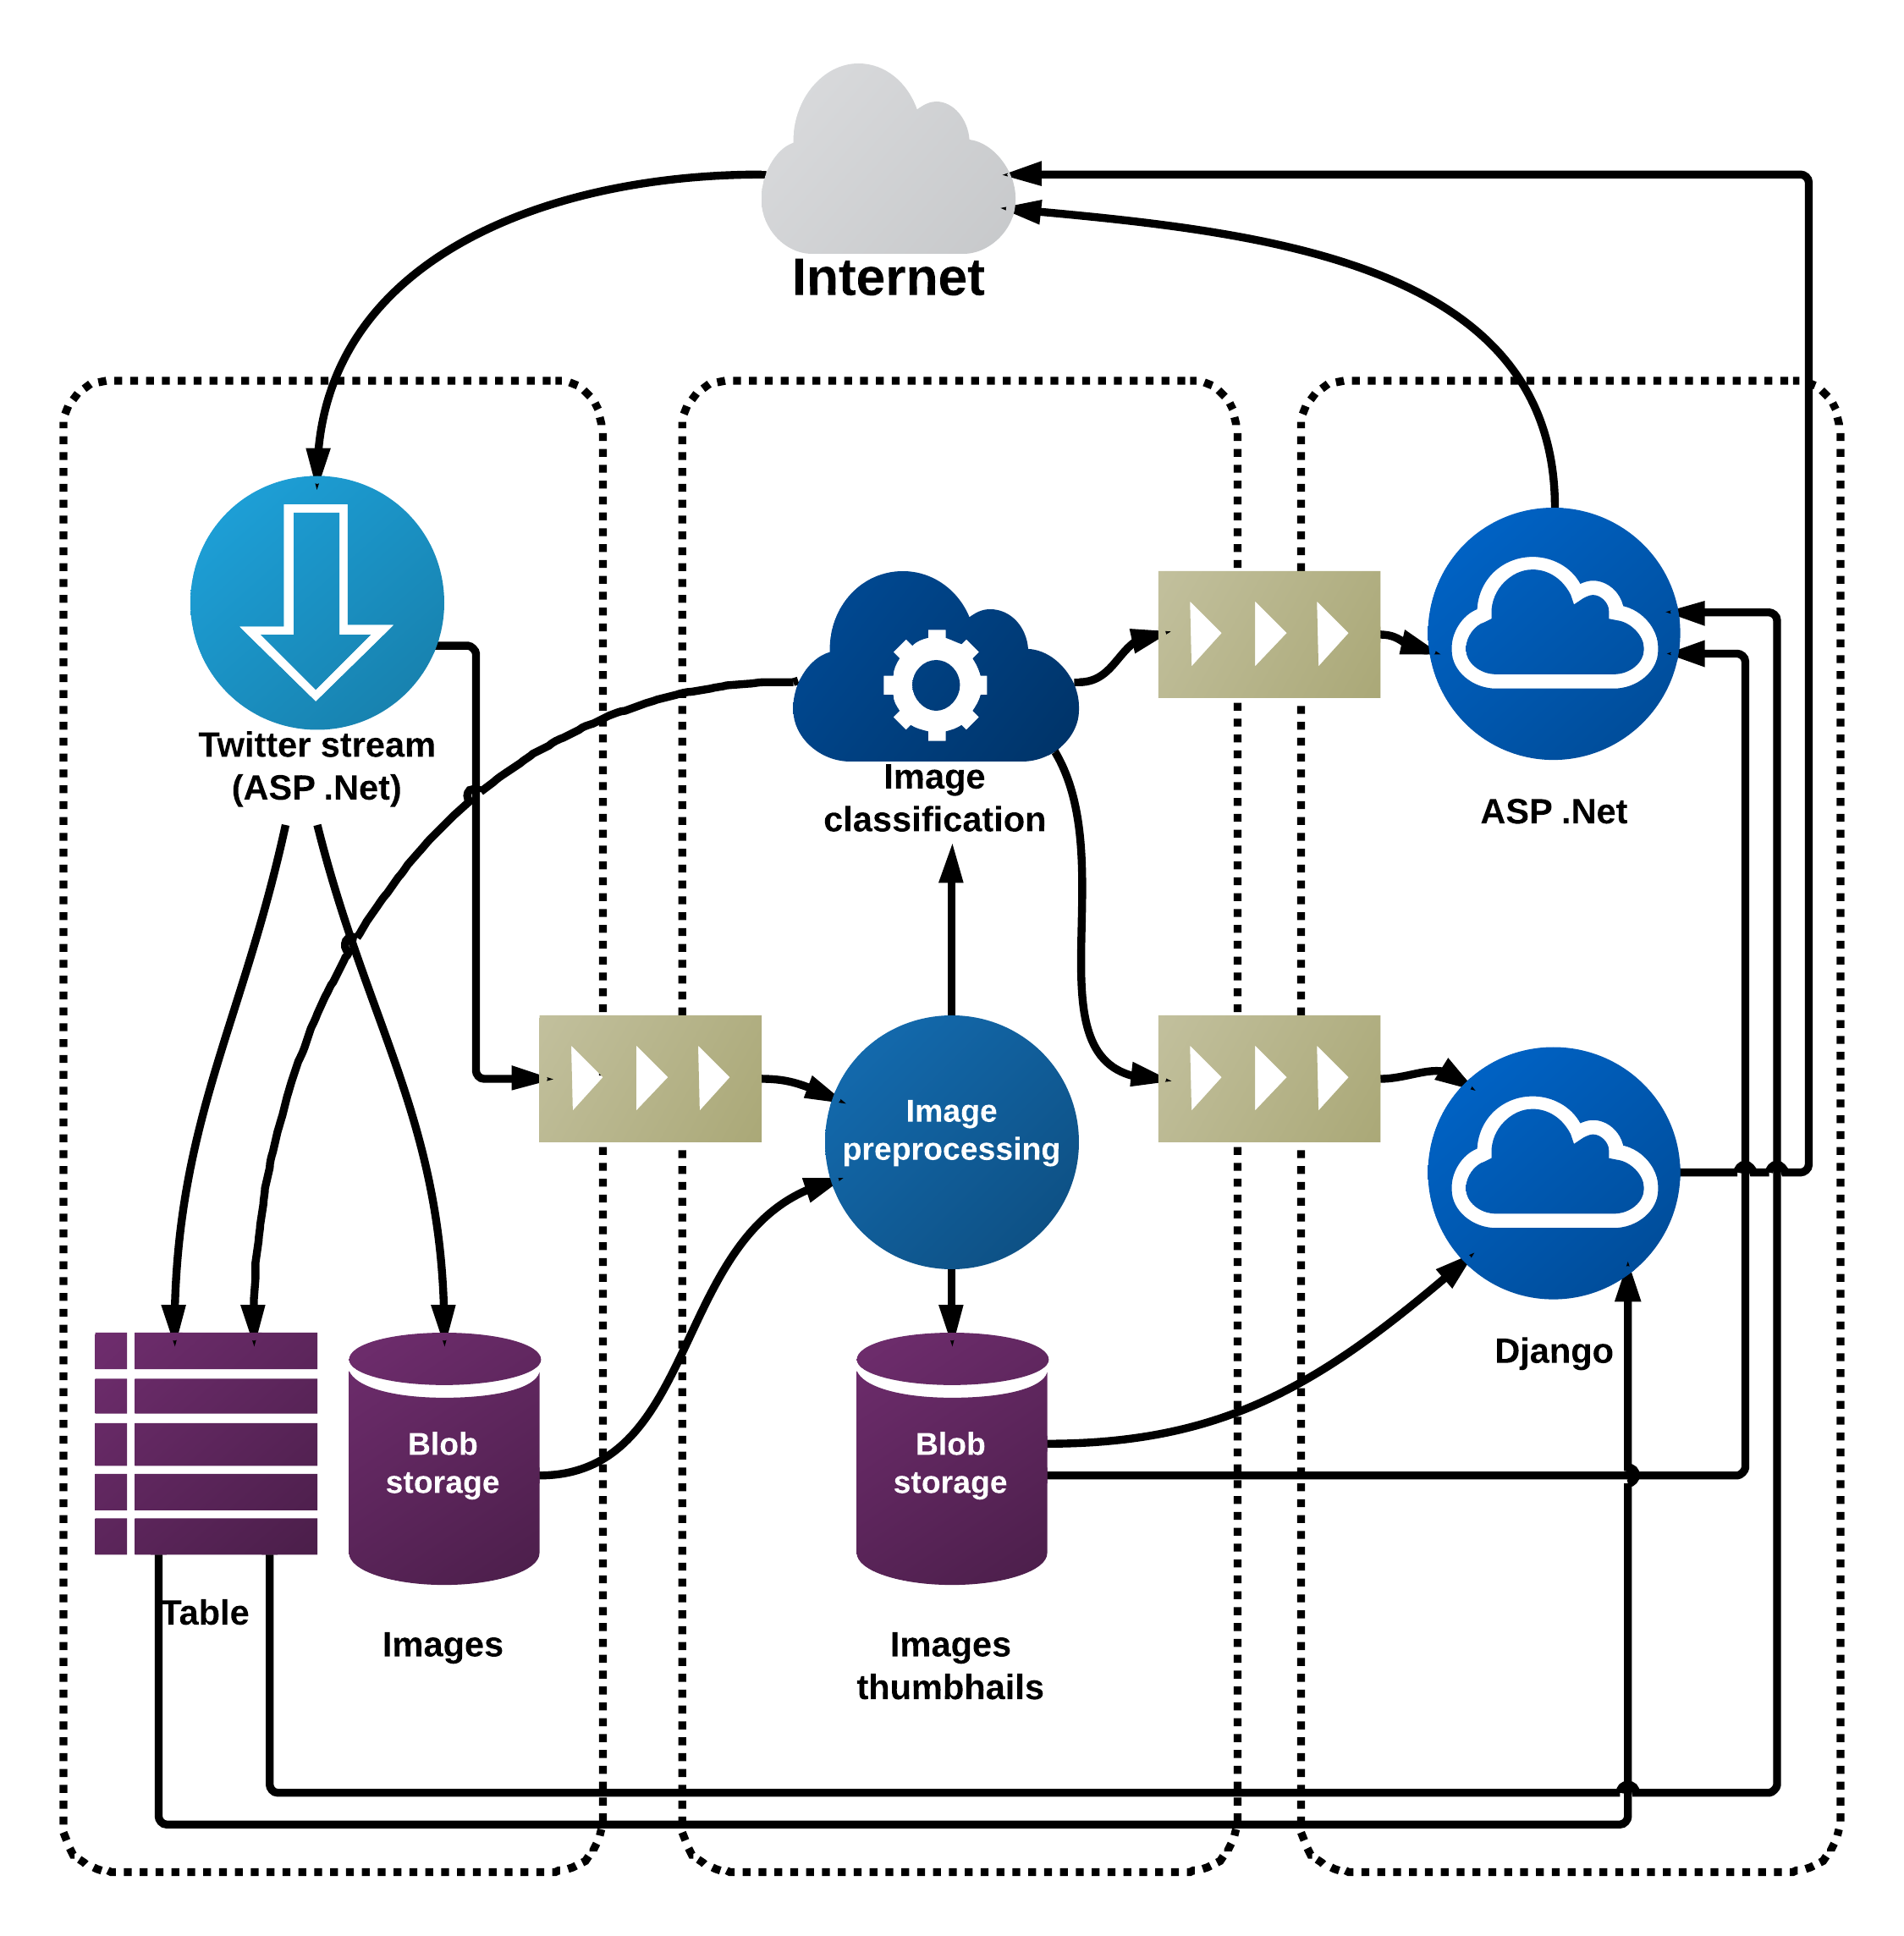
\includegraphics[height=35cm]
                           {../images/scheme}
           \label{fig:desc}
           %% Figure
         \end{tikzfigure}

       }

       \block[
         titleoffsety=-3cm,
         bodyoffsety=-3cm,
         titleoffsetx=3cm,
         bodyoffsetx=3cm,
         titlewidthscale=1.2,
         bodywidthscale=1.2,
       ]
             {Image classification}{
               As classifier for images obtained from Twitter, deep convolutional neural network. Python library Caffe with prebuilt Caffe Reference ImageNet Model (implementation of an ImageNet model trained on ILSVRC-2012) were used.

         Here's short overview of this model: the best validation performance during training was iteration 358,000 with validation accuracy 57.258\% and loss 1.83948.
         This model obtains a top-1 accuracy 57.1\% and a top-5 accuracy 80.2\% on the validation set.~\cite{caffe}
         Max-pooling layers follow first, second, and fifth convolutional layers.
         The number of neurons in each layer is given by 253440, 186624, 64896, 64896, 43264, 4096, 4096, 1000.~\cite{nips2012}

         \begin{tikzfigure}[]
           \includegraphics[height=12cm]
                           {../images/nips2012}
           \label{fig:desc}
           %% Figure
         \end{tikzfigure}

       }

       \column{0.5}

       \block[
         titleoffsety=-5cm,
         bodyoffsety=-5cm,
       ]
           {Web interface}{
         \begin{tikzfigure}[]
           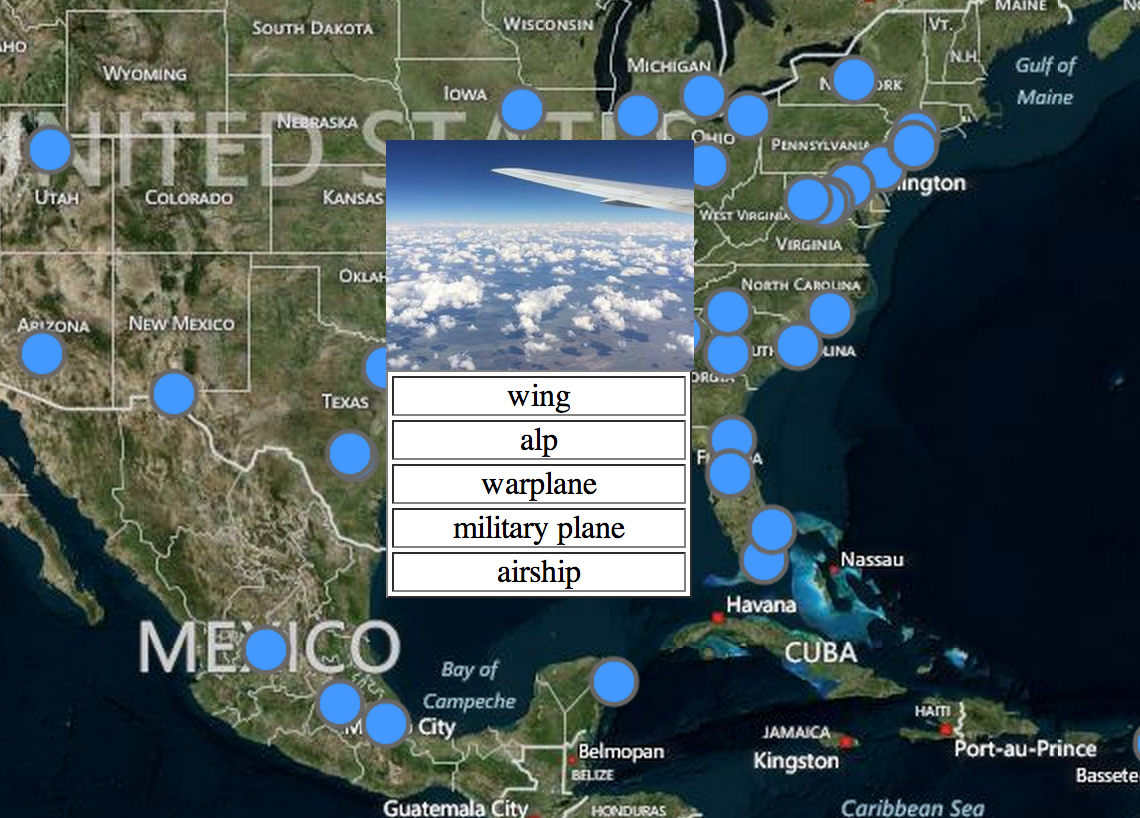
\includegraphics[height=26cm]
                           {../images/airplane}
           \label{fig:desc}
           %% Figure
         \end{tikzfigure}

       }

       \note[
         targetoffsetx=-5cm,
         targetoffsety=-27cm,
         %% rotate=3,
         %% angle=270,
         %% radius=1cm,
         width=.3\textwidth
         %% width=.2\textwidth,
         %% innersep=.4cm
       ]
            {
              Demonstration version is available at the following link:
              \\
              \centering{
              \textbf{\url{http://tweetonmap.azurewebsites.net/}}}\\
              \begin{tikzfigure}[]
                
\includegraphics
                    [height=12cm]
                                {../images/qrcode}
                                \label{fig:desc}
                                %% Figure
              \end{tikzfigure}
            }

       \block[
         titlewidthscale=.8,
         bodywidthscale=.8,
         titleoffsety=-26cm,
         bodyoffsety=-26cm,
         titleoffsetx=3cm,
         bodyoffsetx=3cm
       ]
         {References}{
         \renewcommand{\section}[2]{}%
         %\renewcommand{\chapter}[2]{}% for other classes
         %% \bibliographystyle{plain}
         \bibliography{poster}
       }

     \end{columns}

 \end{document}
